\PassOptionsToPackage{table}{xcolor}
\documentclass[sigconf,anonymous]{acmart}

\AtBeginDocument{%
  \providecommand\BibTeX{{Bib\TeX}}}

\setcopyright{none}
\copyrightyear{2026}
\acmYear{2026}
\acmConference[JCDL '26]{Proceedings of the ACM/IEEE Joint Conference on Digital Libraries}{October 13--16, 2026}{Dallas, Texas, USA}
\acmBooktitle{Proceedings of the ACM/IEEE Joint Conference on Digital Libraries (JCDL '26), October 13--16, 2026, Dallas, Texas, USA}
\acmDOI{}
\acmISBN{}

\usepackage{booktabs}
\usepackage{array}
\usepackage{multirow}
\usepackage{tabularx}
\usepackage{enumitem}
\usepackage{placeins}
\usepackage{xspace}
\setlength{\emergencystretch}{2em}
\raggedbottom

\definecolor{TableBlue}{HTML}{EAF3FA}
\definecolor{TableBlueDark}{HTML}{D8EAF8}
\definecolor{TableGreen}{HTML}{EAF6EA}
\definecolor{TableGreenDark}{HTML}{DDEFD8}
\definecolor{TableRed}{HTML}{F8E6E6}
\definecolor{TableOrange}{HTML}{FFF1D6}
\definecolor{TableGray}{HTML}{F2F2F2}
\definecolor{TableRule}{HTML}{6E6E6E}
\newcolumntype{Y}{>{\raggedright\arraybackslash}X}
\newcommand{\tableheader}{}
\newcommand{\tablesubhead}[2]{\multicolumn{#1}{@{}l}{\textit{#2}}}

\newcommand{\curatability}{curatability\xspace}
\newcommand{\hf}{Hugging Face\xspace}
\newcommand{\llm}{LLM\xspace}
\newcommand{\llms}{LLMs\xspace}

\begin{document}

\title{From Visibility to Curatability: Metadata, Provenance, and Release Evidence for Compact and Derived Open LLM Artifacts}

\begin{abstract}
Open \llm artifacts are often described as available, yet the evidence needed to curate them is distributed across model repositories, papers, model cards, code, and release statements. For digital libraries, this creates a gap between visibility and \curatability: an artifact may be findable without being sufficiently identifiable, linked to scholarship, traceable to upstream models, or accompanied by inspectable release assets. This paper operationalizes \curatability for compact and derived open \llm artifacts through four evidence fields---artifact identity, scholarly linkage, provenance, and release package---and an integrated curation-readiness status. Using a fixed May 2026 snapshot of 191,375 public \hf model repositories and 2,729 scholarly paper records, including 2,214 analysis-set records, we construct linked repository--paper evidence and evaluate it through rule-based normalization, expert audits, and sensitivity checks. The results reveal a sharp visibility-to-curatability funnel: discovery signals are common, but coordinated curation evidence is rare. Matched paper--\hf repository evidence covers 5.6\% of analysis-set paper records; 18.1\% satisfy an operational provenance-plus-release threshold; and only 6.1\% satisfy a stricter joint-evidence threshold. In this scoped public-record corpus, current open \llm publication practices support discovery more readily than digital-library curation. We contribute a reusable measurement framework and a metadata agenda for model hubs, scholarly indexes, and digital libraries.
\end{abstract}

\begin{CCSXML}
<ccs2012>
   <concept>
       <concept_id>10002951.10003227.10003236</concept_id>
       <concept_desc>Information systems~Digital libraries and archives</concept_desc>
       <concept_significance>500</concept_significance>
       </concept>
   <concept>
       <concept_id>10002951.10003260.10003261</concept_id>
       <concept_desc>Information systems~Information extraction</concept_desc>
       <concept_significance>300</concept_significance>
       </concept>
   <concept>
       <concept_id>10002951.10003317.10003318</concept_id>
       <concept_desc>Information systems~Document representation</concept_desc>
       <concept_significance>300</concept_significance>
       </concept>
 </ccs2012>
\end{CCSXML}

\ccsdesc[500]{Information systems~Digital libraries and archives}
\ccsdesc[300]{Information systems~Information extraction}
\ccsdesc[300]{Information systems~Document representation}

\keywords{digital libraries, model repositories, large language models, provenance, metadata, reproducibility, research artifacts, open science}

\maketitle

\section{Introduction}

Digital libraries increasingly steward research objects that live beyond the traditional narrative article \cite{wilkinson2016fair,smith2016softwarecitation,barker2022fair4rs,soilandreyes2022rocrate}. Datasets, software, scripts, model weights, evaluation assets, and external repositories have become fundamental components of the scholarly record, ensuring that computational findings remain inspectable, reusable, and preservable. Open \llm research intensifies this paradigm shift, as a single paper may release a small model, a LoRA adapter, a quantized checkpoint, a merged model, a distilled student, or a deployment package whose operational meaning depends heavily on upstream dependencies and visible release assets. These compact and derived artifacts are rarely contained within a single monolithic record, existing instead as scattered traces across article text, \hf repositories, model cards, source code links, platform metadata fields, family names, and release statements. Institutional curation must therefore address a distributed scholarly record rather than an isolated paper or repository.

This distribution creates a practical curation problem because public visibility does not automatically guarantee curation readiness. The artifact is not necessarily hidden; it may be visible in several places at once. Yet a future curator may still be unable to decide what object should be cited, which repository is the release rather than a dependency, which upstream relation should be recorded, or which assets should be selected for preservation triage. A visible model-hub link may help a researcher locate an asset, but it rarely clarifies whether the target repository represents an official release, a baseline dependency, a temporary checkpoint package, or a third-party derivative. Similarly, a referenced model family name can identify the target artifact, an upstream base checkpoint, a teacher model, an experimental baseline, or general background context. In this sense, the risk is not only artifact loss but evidence loss: public traces exist, while the relations that make them curatable remain underspecified. The artifact may remain online, but the evidence needed to cite, attribute, trace, reuse, and preserve it can still disappear into untyped links and ambiguous release statements.

Existing literature provides critical foundational insights without offering a collection-scale assessment of this systemic record problem. Prior work on model cards, datasheets, model openness, reproducibility, software citation, data citation, research-object packaging, and context-based URL classification demonstrates that computational artifacts require structured documentation rather than binary availability metrics \cite{gebru2021datasheets,mitchell2019modelcards,pineau2021reproducibility,bommasani2023fmi,white2024mof,salsabil2025context}. Empirical studies of model hubs and asset reuse further clarify how these models circulate through open-source artificial intelligence communities \cite{jiang2023ptmreuse,taraghi2024modelreuse,osborne2024aicommunity}. Most of these investigations, however, evaluate only one record type at a time, focusing exclusively on isolated papers, individual URLs, code repositories, distinct model cards, datasets, or platform-specific model-hub behavior. Digital preservation systems still lack empirical evidence demonstrating how papers, model hubs, model cards, and release links interact to support or hinder the systematic curation of compact and derived open \llm artifacts.

We address this empirical gap by operationalizing \curatability as a record-level measure of curation readiness. In this study, a curatable public record provides sufficient evidence to determine the artifact's operational role, its record-supported scholarly linkage, its upstream model evidence, and its visible release assets available for inspection and preservation triage. Utilizing a fixed May 2026 snapshot, we evaluate 191,375 public \hf model repositories and 2,729 scholarly paper records, filtering the literature into a core analysis set of 2,214 papers. Our measurement pipeline constructs linked repository-paper evidence by normalizing repository metadata, paper-side links, alignment signals, provenance evidence, and release-package fields, incorporating expert audits and sensitivity checks to calibrate boundary conditions.

Cross-system measurements reveal a severe drop-off from initial asset visibility to ultimate curation readiness. Public records successfully establish a broad discovery layer, with 90.7\% of analysis-set papers containing at least one useful curation signal. The proportion of viable records contracts dramatically when curation requires multiple evidence fields to co-occur. Explicitly matched paper-to-\hf repository evidence covers only 5.6\% of the analysis-set papers. An operational threshold requiring usable provenance alongside concrete release evidence identifies 18.1\% of records, whereas a stricter threshold requiring usable provenance, asset-level release evidence, and a direct linkage signal identifies only 6.1\% of the corpus. Systemic fragmentation across metadata platforms, rather than an absolute absence of public artifacts, forms the primary bottleneck to preservation-aware digital-library curation.

Primary contributions of this work encompass three distinct dimensions:

\begin{itemize}[leftmargin=*]
    \item \textbf{Digital-library framing.} We establish a curation framing that repositions compact and derived open \llm artifacts as distributed scholarly objects.
    \item \textbf{Audited empirical record construction.} We present a linked record construction for evaluating artifact identity, scholarly linkage, upstream evidence, release-package evidence, and integrated curation readiness.
    \item \textbf{Metadata and interface recommendations.} We translate these empirical insights into concrete interventions for model hubs, scholarly indexes, and digital libraries, detailing fields for typed artifact roles, bidirectional paper--repository relations, upstream relation types, provenance evidence tiers, and structured release-package fields.
\end{itemize}

These findings offer a constructive implication for open science, demonstrating that current infrastructure supports broad public visibility, while the next milestone requires rendering public evidence sufficiently structured to support systematic citation, reuse, provenance tracking, and preservation triage.

\section{Curation Framework}
\label{sec:framework}

Investigating the boundaries of digital library curation requires focusing on what curators can reliably assert when open \llm artifact metadata is scattered across model hubs and scholarly literature. Rather than attempting to reconstruct the exhaustive training history of an artifact or executing the model to verify performance, our evaluation measures public-record sufficiency: whether visible traces support an auditable curation record. Public traces include model repository pages, model cards, links or textual mentions within papers, upstream model fields, family labels, code repository links, and formal release statements. Retaining the explicit source, specific role, and evidentiary strength of these traces allows digital libraries to convert surface-level visibility into verifiable curation evidence, following broader work on FAIR artifacts, software citation, research-object packaging, and context-sensitive scholarly links~\cite{wilkinson2016fair,smith2016softwarecitation,soilandreyes2022rocrate,salsabil2025context}.

Synthesizing a single paper record with its corresponding model-hub repositories allows curators to construct an evidence-backed curation record. Such a record addresses four core dimensions: what the artifact is, how it connects to specific scholarship, what upstream dependencies or derivation relations are publicly supported, and which release assets are visible for preservation triage. These dimensions draw from model documentation, provenance, and reproducibility research, where artifact identity, context, derivation, and inspectable release materials are treated as separate metadata requirements rather than a single availability flag~\cite{mitchell2019modelcards,gebru2021datasheets,moreau2013prov,pineau2021reproducibility}. Incorporating an integrated curatability status explicitly marks whether these distinct evidentiary fields co-occur within a single record. Shifting the assessment framework from binary accessibility metrics, such as link presence or download capability, allows digital libraries to evaluate record sufficiency rather than mere public visibility.

We therefore evaluate five curation functions. Artifact identity asks whether public records distinguish base checkpoints, fine-tunes, adapters, merges, quantized packages, distilled students, and deployment artifacts. Scholarly linkage asks whether the artifact can be connected to papers, repositories, owners, dates, licenses, and task contexts. Provenance sufficiency asks whether upstream evidence is explicit or canonical, inventory-backed, contextual, or missing, following provenance research that separates traceable derivation relations from weaker contextual evidence~\cite{moreau2013prov,davidson2008provenance,herschel2017survey}. Release-package readiness asks whether visible records expose code, scripts, recipes, checkpoints, adapters, data, or evaluation assets rather than only release intentions, reflecting reproducibility work showing that access statements alone do not establish practical reuse or rerun readiness~\cite{dodge2019show,pineau2021reproducibility,akella2023effort}. Integrated curatability asks whether these fields co-occur in one auditable record.

Two operational boundaries define the scope of this framework. First, the study measures curation claims supported strictly by public records rather than trying to map the absolute, exhaustive genealogy of an artifact. True model lineage frequently depends on private training logs, local commit histories, unreleased intermediate checkpoints, or implicit developer knowledge, forcing digital libraries to rely on visible records to establish auditable metadata. This boundary is especially important for open-model reuse, where public records may expose family names, model-card fields, or downstream adaptation signals without fully specifying the underlying dependency relation~\cite{jiang2023ptmreuse,taraghi2024modelreuse,white2024mof}. Second, evidence must be tiered rather than treating all public signals as equivalent. Model-card fields, paper-side links, family mentions, and formal release statements serve fundamentally different curation purposes and cannot be used interchangeably~\cite{mitchell2019modelcards,pepe2024hfdocs,kadasi2025modelhubs,salsabil2025context}. Preserving the alignment among evidence sources, audit checks, and target uses guides the empirical measurement design across five core parameters: identity, linkage, provenance, release packages, and integrated curatability.

\section{Related Work}
\label{sec:related}

\subsection{Research Artifacts and Scholarly Records}
Modern open-science and digital-library research increasingly treats datasets, software, URLs, code repositories, and packaged research objects as core elements of the broader scholarly record~\cite{wilkinson2016fair,datacitation2014joint,smith2016softwarecitation,lamprecht2020fairsoftware,katz2021freshfairsoftware,barker2022fair4rs,soilandreyes2022rocrate}.
Frameworks such as the FAIR data principles, software citation standards, FAIR research software, and RO-Crate protocols emphasize that computational artifacts require persistent identifiers, explicit authorship, licenses, dependencies, and contextual metadata instead of simple access hyperlinks~\cite{wilkinson2016fair,datacitation2014joint,smith2016softwarecitation,lamprecht2020fairsoftware,katz2021freshfairsoftware,barker2022fair4rs,soilandreyes2022rocrate}.
Analysis of scholarly URLs similarly reveals that a visible hyperlink falls short of a functional curation record because its surrounding textual context must be interpreted before the link can support metadata generation, discovery, or long-term preservation choices~\cite{salsabil2025context}.
Existing scholarship establishes the bibliographic value of detailed artifact descriptions while primarily focusing on established artifact classes such as standalone datasets, software packages, URLs, or structured research objects.
Distributed record fragmentation becomes more pronounced for compact or derived open \llm artifacts because their operational identity, scholarly relationships, upstream dependencies, and release components may be scattered across papers, hub repositories, model cards, code repositories, and developer statements~\cite{mitchell2019modelcards,pepe2024hfdocs,kadasi2025modelhubs,jiang2023ptmreuse,taraghi2024modelreuse}.
Building on these foundations, our study asks when fragmented public traces mature into sufficient evidence for institutional digital-library curation.

\subsection{Reuse, Reproducibility, and Release Packages}
Existing literature on repository reuse and computational reproducibility draws a sharp distinction between baseline availability and functional reuse~\cite{shiri2023reuse,stodden2014implementing,akella2023effort,dodge2019show,pineau2021reproducibility}.
Investigations into repository interfaces demonstrate that evaluating reuse requires tracking how digital objects are shared, transformed, and recontextualized~\cite{shiri2023reuse}.
Methodological studies and reproducibility reporting programs similarly show that publishing raw source code does not reflect the full effort required to inspect, rerun, or validate computational findings; auxiliary artifacts, documentation, environments, and procedural details also matter~\cite{stodden2014implementing,akella2023effort,dodge2019show,pineau2021reproducibility}.
This broader view motivates evaluating release evidence as a multi-layered package rather than classifying availability through a simple open-or-closed variable.
Emerging open \llm variants introduce distribution patterns that are not well captured by generic software availability fields: a single record may expose training code, fine-tuning recipes, checkpoint weights, LoRA adapters, quantized files, evaluation assets, or only an unfulfilled statement of intent~\cite{jiang2023ptmreuse,taraghi2024modelreuse,white2024mof}.
Grounded in this multi-tiered perspective, our release-package hierarchy categorizes which visible assets a publication record exposes for inspection and curation without assuming that those assets are executable or complete.

\subsection{Provenance and Derived-Model Relations}
Provenance frameworks have long been foundational to digital-library architectures, scientific workflows, and computational reproducibility~\cite{moreau2013prov,davidson2008provenance,herschel2017survey}.
Standardized representations such as the W3C PROV model formalize lineage by mapping entities, activities, and agents to explain how research artifacts are derived and produced~\cite{moreau2013prov}.
Digital-library systems further illustrate how provenance tracking can be integrated into document-analysis workflows so that generated outputs, processing steps, and analytical decisions remain traceable~\cite{rauch2025ontextract}.
Open \llm deployments introduce a related but more relation-specific challenge.
A derived or compressed model variant may depend on an upstream artifact as a base checkpoint, teacher for distillation, adapter target, merge source, quantization source, evaluator, or baseline~\cite{jiang2023ptmreuse,taraghi2024modelreuse,white2024mof}.
Available public records frequently mention broad model-family names or contextual references that aid basic discovery without encoding an explicit, machine-readable upstream relationship.
Addressing this limitation requires treating provenance as a tiered spectrum of public evidence, where broad family-level signals support catalog organization while rigorous curation demands canonical upstream declarations and explicit relationship types.

\subsection{Model Documentation, Model Hubs, and Open AI Infrastructure}
Documentation paradigms such as model cards and structured datasheets provide influential templates for recording the properties of machine-learning models and datasets~\cite{mitchell2019modelcards,crisan2022interactive,shen2022modelcardtoolkit,gebru2021datasheets}.
Frameworks such as Data Cards and the Croissant format extend this documentation agenda by encoding data assets and ML-ready resources as structured metadata objects~\cite{pushkarna2022datacards,akhtar2024croissant}.
Quantitative analyses of active model repositories reveal that documentation practices vary substantially across communities, particularly in how authors report licensing, training datasets, model properties, and reuse guidance~\cite{liang2024modelcards,pepe2024hfdocs,kadasi2025modelhubs}.
Independent tracking of \hf repository activity further demonstrates how pretrained models undergo reuse, adaptation, and open-source distribution throughout AI developer communities~\cite{jiang2023ptmreuse,taraghi2024modelreuse,osborne2024aicommunity}.
Collaborative transparency frameworks similarly emphasize that openness depends on multiple technical components rather than model weights alone~\cite{bommasani2023fmi,white2024mof}.
Prior landscape evaluations map how infrastructure platforms distribute and govern AI artifacts, yet they typically isolate a single documentation layer such as a model card, repository field, reuse network, or openness checklist.
Our research shifts the unit of analysis toward the cross-system scholarly record.
Connecting repository metadata with scholarly publications allows us to ask what existing public records reveal about artifact identity, paper-to-repository linkage, upstream-evidence claims, inspectable release assets, and integrated curation readiness.

\section{Data and Measurement Design}
\label{sec:methods}

This section explains how we turn distributed public traces into auditable record-level measures. Figure~\ref{fig:pipeline} summarizes the pipeline. The study starts from two public evidence sources---model-hub repository records and scholarly paper records---and converts visible traces into typed fields for artifact identity, scholarly linkage, provenance, release packages, and integrated curation readiness. Three principles guide the measurement. First, the source of each trace is preserved, because a model-card field, a paper-side link, and a family mention support different claims. Second, denominators are kept separate, because repository records, paper records, and record-supported artifact claims are not interchangeable. Third, judgment-sensitive fields are calibrated through expert audits and sensitivity checks, so strict metadata claims can be separated from broader discovery or collection-organization signals.

\begin{figure*}[!tbp]
    \centering
    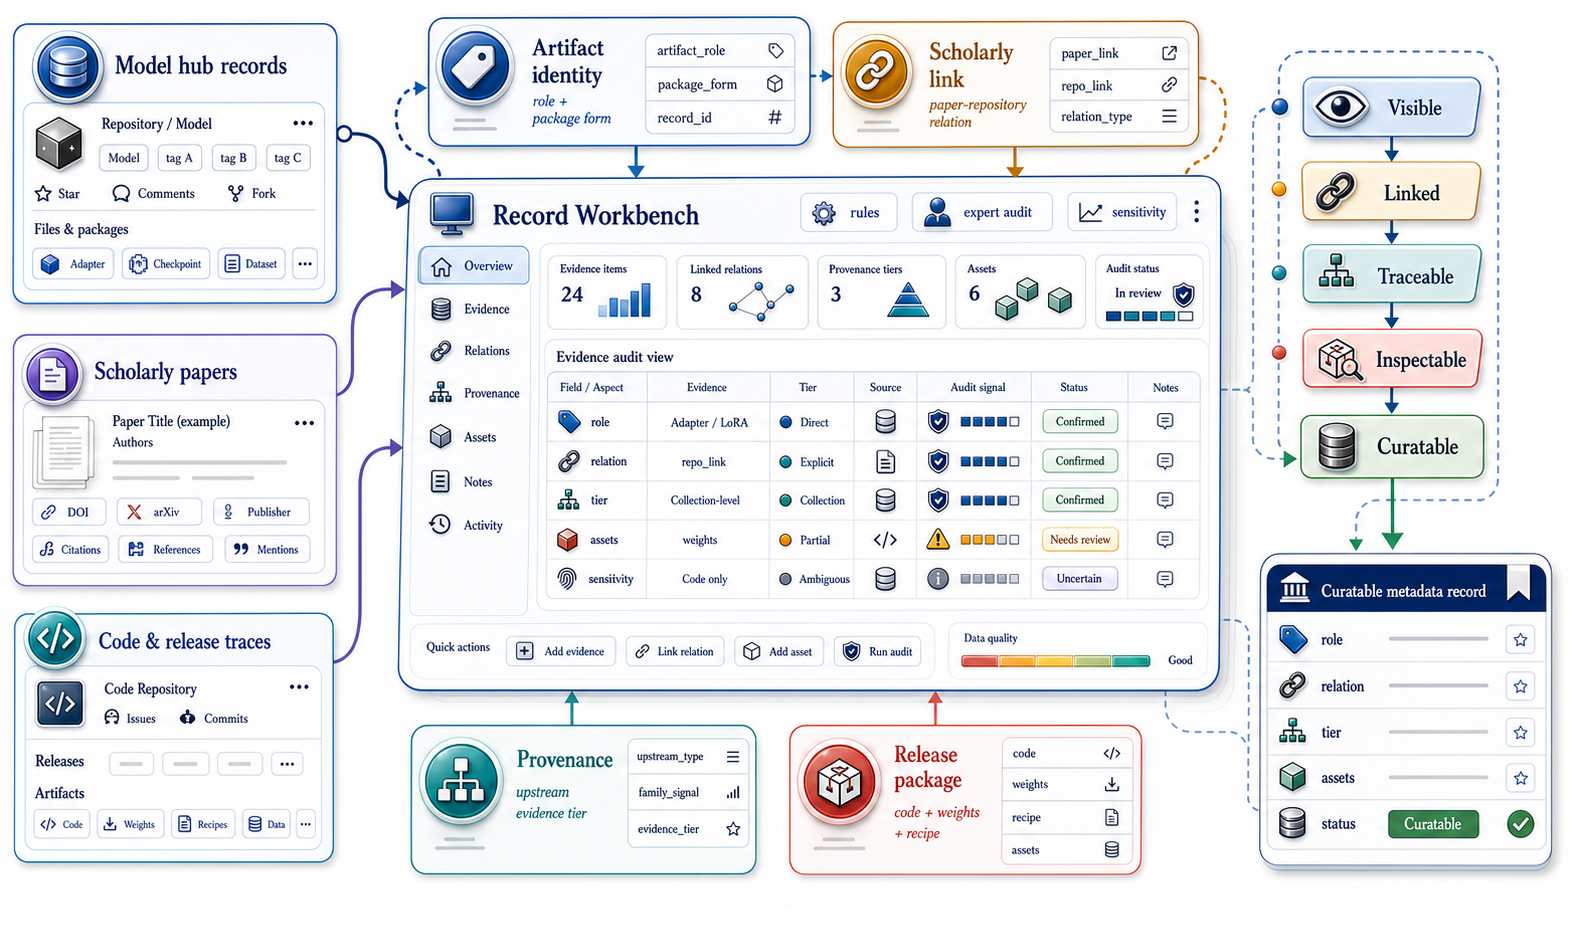
\includegraphics[width=\textwidth]{figures/fig1_overview_gpt_image2_icon_polished_library_crop.png}
    \caption{Overview of the visibility-to-curatability measurement design. Public model-hub, paper, code, and release traces are converted into four typed evidence fields: artifact identity, scholarly linkage, provenance, and release package. Normalization, expert audits, and sensitivity checks distinguish strict evidence, collection-level evidence, and weak or missing evidence before assigning an integrated curation-readiness status.}
    \Description{A workflow diagram with four panels: public traces, evidence extraction, normalization and audit, and curatability decision.}
    \label{fig:pipeline}
\end{figure*}

\begin{table*}[!tbp]
\centering
\caption{Measurement constructs and checks. Each row maps one curation construct to its denominator, signal, calibration check, and supported claim.}
\label{tab:measurement-constructs}
\small
\setlength{\tabcolsep}{3.6pt}
\renewcommand{\arraystretch}{1.08}
\begin{tabular}{@{}p{0.17\linewidth}p{0.18\linewidth}p{0.22\linewidth}p{0.17\linewidth}p{0.18\linewidth}@{}}
\toprule
\textbf{Construct} & \textbf{Unit} & \textbf{Signal} & \textbf{Check} & \textbf{Output claim} \\
\midrule
Artifact identity & 191,375 repos & Role + package form & 300-role audit & Typed identity \\
Scholarly linkage & Repos + 2,214 papers & HF/GitHub links; backlinks & Alignment split & Typed relation \\
Provenance & 2,214 papers & Upstream tier $P$ & 200-row audit & Upstream claim \\
Release package & 2,214 papers & Release tier $R$ & 50-URL audit & Visible assets \\
\textbf{Integrated} & 2,214 papers & \textbf{P/R/L rule} & Sensitivity & \textbf{Readiness status} \\
\bottomrule
\end{tabular}
\renewcommand{\arraystretch}{1.0}
\end{table*}


\subsection{Corpus Construction and Scope}

We built the dataset in four steps: repository collection, paper collection, evidence coding, and validation. The repository collection is a scoped May 2026 query-based snapshot of 191,375 public \hf model repositories. It is designed to capture public records likely to describe compact or derived open \llm artifacts, rather than to serve as a census of all \hf repositories. Query terms were grouped into five buckets---size or compactness, deployment format, derivation or tuning, domain/language/task, and model-family names. Query-bucket sensitivity analysis reports how this scoping affects repository-side measurements.

The repository snapshot contains repository identifiers, owners, creation timestamps, tags, model-family labels, upstream model fields, arXiv references, task descriptors, domain descriptors, and project-inferred artifact role and package-form fields. We treat artifact role and package form as audited inference fields derived from repository metadata and tags. The role taxonomy includes base, fine-tune, adapter/LoRA, merge/mixed, and quantized/deployment records. Package form captures distribution signals such as adapter-only, quantized, converted, checkpoint-complete, code-only, or multi-asset release packaging.

The scholarly corpus combines records from OpenAlex, arXiv metadata, and venue-derived paper lists. After merging and deduplication, it contains 2,729 paper records, corresponding to 2,722 works. We filter these records into a main analysis set of 2,214 paper records, corresponding to 2,208 works, that centrally study compact or derived open \llm artifacts. A paper enters the analysis set when it introduces, adapts, compresses, quantizes, distills, fine-tunes, evaluates, or deploys a compact or derived model artifact as a central research object. Application-only pipelines, general benchmarks, and papers that merely use \llms as tools are excluded unless the compact or derived artifact is itself the object of study.

This scope is operational rather than parameter-count based. ``Compact'' includes strict small models and deployment-oriented compact models. ``Derived'' includes compressed, quantized, distilled, PEFT/adapted, merged, domain-specialized, and evaluation- or deployment-oriented artifacts whose interpretation depends on upstream models or released assets. The anonymized supplementary package lists the query buckets, input sources, construction rules, and derived files used for the reported figures and tables.

\subsection{Evidence Fields and Units of Analysis}

The study uses three denominators. Repository-level percentages describe records in the fixed \hf snapshot. Paper-level percentages describe the 2,214 analysis-set paper records. Artifact-level language refers to curation claims supported by those public records, not to a census of unique model artifacts. This separation is necessary because a paper may discuss multiple model objects, a repository may package an artifact derived from another repository, and the same family name may appear as a target model, parent, teacher, baseline, evaluator, or background context.

Each evidence field supports a distinct curation claim. For scholarly linkage, we keep paper-side \hf links, paper-side GitHub or code-hosting links, repository-side arXiv references, exact model mentions, model-card references, and low-confidence family/size matches as separate signals. These signals differ in evidentiary strength: a paper-side link, a repository backlink, and a matched model mention do not support the same bibliographic claim. In the integrated rubric, the linkage component $L\geq1$ is triggered by one direct alignment signal: an exact \hf edge, an explicit paper-side \hf link, or an explicit paper-side GitHub/code-hosting link. Low-confidence fuzzy matches are retained for sensitivity analysis but do not by themselves satisfy this direct-linkage threshold.

For provenance, we assign each analysis-set paper record to the strongest upstream-evidence tier supported by public records. Stronger tiers require explicit or canonical upstream evidence, such as a visible upstream-model field, a paper statement that the artifact is based on a named checkpoint, or a matched repository whose upstream relation is visible. Lower tiers capture curated-inventory family support, weak contextual family clues, or no usable signal. A paper-repository link may help locate the relevant record, but it supports provenance only when the linked record or paper text exposes an upstream relation. This tiering measures public-record sufficiency, not complete model genealogy.

For release packages, we use a five-level hierarchy: no explicit release signal; stated or incomplete release signal; code, scripts, or recipe; checkpoint, adapter, data, or evaluation asset; and multiple assets or a full recipe. The hierarchy treats openness as visible record evidence for curation. It does not claim that released assets execute successfully or reproduce the reported results.

Table~\ref{tab:measurement-constructs} summarizes the relationship among constructs, denominators, evidence sources, calibration checks, and curation claims. The design keeps visible traces typed: a model-card field, a paper-side link, a family mention, and a release statement are not interchangeable records. They become useful for digital-library curation when their source, calibration evidence, and supported use are retained together.

\subsection{Coding, Calibration, and Audits}

The dataset combines structured Web records with unstructured scholarly text, so we separate three classes of fields. Native fields, such as repository identifiers, timestamps, tags, upstream-model fields, arXiv references, paper metadata, and URLs, are treated as observed public metadata. Rule-derived fields, such as query buckets, denominators, alignment tiers, release-evidence levels, and curatability scores, are generated by deterministic scripts from documented inputs. Judgment-sensitive fields, such as paper inclusion, artifact role, provenance sufficiency, and release-evidence interpretation, are calibrated through expert audits or agreement checks.

LLM-assisted coding is used only as an evidence-extraction aid for paper text. The prompts return structured candidate fields and short supporting excerpts from extracted paper sections. No reported aggregate label is taken directly from a generative output. Final analytical fields are produced after schema validation, rule-based normalization, curated-inventory matching, link-table resolution, and expert-calibrated decision boundaries. The prompt template, extraction schema, model settings, raw candidate outputs, and detailed agreement statistics are documented in the supplementary reproducibility files. The main JCDL measures are artifact role, scholarly linkage, provenance sufficiency, release-package evidence, and integrated curatability.

We report three construct-specific audit layers in the main text. A balanced repository-role audit reviews 300 repositories, with 60 predicted records per role, and checks whether public metadata supports the assigned primary role or suggests a role change or package-form ambiguity. A targeted upstream-evidence audit reviews 200 paper-level provenance rows and distinguishes strict unique-primary support from usable family-level support. A release audit reviews 50 URL or asset-signal rows and checks whether extracted release categories match visible public evidence. These samples calibrate boundary interpretation rather than estimate corpus-wide prevalence; aggregate labels remain rule-based and reproducible. We also report query-bucket sensitivity, alignment-signal decomposition, and curatability-threshold sensitivity.

\begin{table*}[!tbp]
\centering
\caption{Expert-audit outcomes with Wilson 95\% intervals. Audits calibrate boundary decisions rather than estimate population prevalence.}
\label{tab:audit-wilson-ci}
\small
\setlength{\tabcolsep}{5pt}
\renewcommand{\arraystretch}{1.14}
\begin{tabularx}{0.94\textwidth}{@{}p{0.16\textwidth}p{0.21\textwidth}cp{0.18\textwidth}Y@{}}
\toprule
\textbf{Audit layer} & \textbf{Boundary checked} & \textbf{Count} & \textbf{Estimate (95\% CI)} & \textbf{Audit implication} \\
\midrule
Repository role & Strict role support & 256/300 & \cellcolor{TableGreen}\textbf{85.3\%} [80.9, 88.9] & Artifact-role labels are stable \\
\midrule
Upstream evidence & Strict unique-primary & 56/200 & \cellcolor{TableRed}28.0\% [22.2, 34.6] & Strict lineage claims stay conservative \\
 & Usable family-level & 158/200 & \cellcolor{TableGreen}\textbf{79.0\%} [72.8, 84.1] & Family-level grouping is usable \\
\midrule
Release evidence & URL/asset category retained & 50/50 & \cellcolor{TableGreen}\textbf{100.0\%} [92.9, 100.0] & Release categories are stable \\
\bottomrule
\end{tabularx}
\renewcommand{\arraystretch}{1.0}
\end{table*}


\subsection{Integrated Curatability Rubric}

We synthesize provenance, release, and linkage evidence into an integrated curatability rubric. The rubric does not rank model quality, adoption, or executable reproducibility. Each threshold corresponds to a distinct curator task: discovery, grouped inspection, bibliographic control, provenance-aware preservation triage, or multi-asset review.

The provenance component ranges from 0 to 3: no usable provenance, weak contextual clue, curated-inventory family support, and exact or canonical upstream signal. The release component ranges from 0 to 4 using the hierarchy above. The linkage component ranges from 0 to 2: no direct signal, one direct linkage signal, and two or more signals. A \textit{discovery-ready} record contains at least one useful provenance, release, or link signal. The \textit{operational P+R} threshold requires usable provenance and code/recipe-or-stronger release evidence. The \textit{operational+link} sensitivity adds at least one direct linkage signal. The \textit{high-curatability} threshold requires usable provenance, asset-level release evidence, and at least one direct linkage signal. The \textit{preservation-review candidate} threshold further requires a multi-asset or full-recipe release package.

For example, a paper record with an explicit \hf link, a visible upstream base-model relation, and released adapter weights receives link evidence, usable provenance evidence, and asset-level release evidence; it satisfies the high-curatability threshold. A paper record with only a family name and a statement that resources will be released remains useful for discovery, but falls below the operational P+R threshold because the release package is not concrete.

The threshold ladder maps each numerical rule to a curator task. Provenance score $P\geq2$ supports at least family-level collection organization or attribution triage. Release score $R\geq2$ means that code, scripts, or recipe evidence is visible for inspection. Release score $R\geq3$ adds an asset-level package such as a checkpoint, adapter, data, or evaluation asset. Linkage score $L\geq1$ supports bibliographic control through a direct alignment signal. The strictest rule, $P\geq2$, $R\geq4$, and $L\geq1$, identifies preservation-review candidates with multi-asset packages; it is still not an execution test.

The operational+link sensitivity changes the count only marginally because almost all records satisfying $P\geq2$ and $R\geq2$ also contain at least one direct alignment signal under the broad $L$ definition. This is why the main bottleneck is not link evidence after provenance and concrete release evidence are already present, but the co-occurrence of usable provenance and concrete release evidence in the first place.

\section{Results}
\label{sec:results}

The results show a visibility-to-curatability funnel. Public records often support discovery and collection organization, but the record set narrows as curation requires stronger combinations of evidence: 90.7\% of analysis-set paper records are discovery-ready; 18.1\% combine usable provenance with concrete code, recipe, or stronger release evidence; and 6.1\% additionally satisfy the high-curatability requirement of direct linkage plus asset-level or multi-asset release evidence. Table~\ref{tab:key-results} summarizes the evidence ingredients and composite thresholds. The five RQs follow the curation workflow. RQ1--RQ4 explain why identity, linkage, provenance, and release evidence each exist in public records but cannot be substituted for one another; RQ5 diagnoses where these fields fail to co-occur.

\begin{table*}[!tbp]
\centering
\caption{Headline evidence components and curation thresholds. Counts use 2,214 analysis-set paper records. $P$, $R$, and $L$ denote provenance, release-package, and direct-linkage scores.}
\label{tab:key-results}
\normalsize
\setlength{\tabcolsep}{6pt}
\renewcommand{\arraystretch}{1.08}
\begin{tabular*}{\textwidth}{@{\extracolsep{\fill}}llrrl@{}}
\toprule
\textbf{Group} & \textbf{Evidence or threshold} & \textbf{Count} & \textbf{Share} & \textbf{Takeaway} \\
\midrule
\multicolumn{5}{@{}l}{\textit{Evidence components}} \\
\cmidrule(lr){1-5}
Linkage & Matched paper--HF repo & 124 / 2,214 & 5.6\% & Direct relation rare \\
Provenance & Inventory-backed family & 1,009 / 2,214 & 45.6\% & Grouping, not lineage \\
Release & Code/asset evidence ($R\geq2$) & 793 / 2,214 & 35.8\% & Concrete release uneven \\
\midrule
\multicolumn{5}{@{}l}{\textit{Curation-readiness thresholds}} \\
\cmidrule(lr){1-5}
Discovery-ready & Any useful signal & 2,008 / 2,214 & \textbf{90.7\%} & Broad visibility \\
Operational P+R & $P\geq2, R\geq2$ & 401 / 2,214 & \textbf{18.1\%} & Usable P + release \\
High-curatability & $P\geq2, R\geq3, L\geq1$ & 136 / 2,214 & \textbf{6.1\%} & Joint evidence bottleneck \\
Preservation-review & $P\geq2, R\geq4, L\geq1$ & 50 / 2,214 & 2.3\% & Multi-asset subset \\
\bottomrule
\end{tabular*}
\renewcommand{\arraystretch}{1.0}
\end{table*}


\subsection{RQ1: Can Repository Records Identify Artifact Roles?}

Repository records provide broad coverage for artifact typing, but confidence is uneven across roles. In the fixed \hf snapshot, our pipeline assigns project-inferred artifact-role and package-form labels to all 191,375 repository records from public metadata and tags. Figure~\ref{fig:metadata}a shows which curation fields are broadly visible and which remain sparse: task descriptors, family labels, upstream fields, and license signals appear frequently, while scholarly references and domain descriptors remain much less complete. Figure~\ref{fig:metadata}b shows that role typing is stable for several derived-artifact classes, while base and merge/mixed records require richer package-form information.

\begin{figure*}[!tbp]
    \centering
    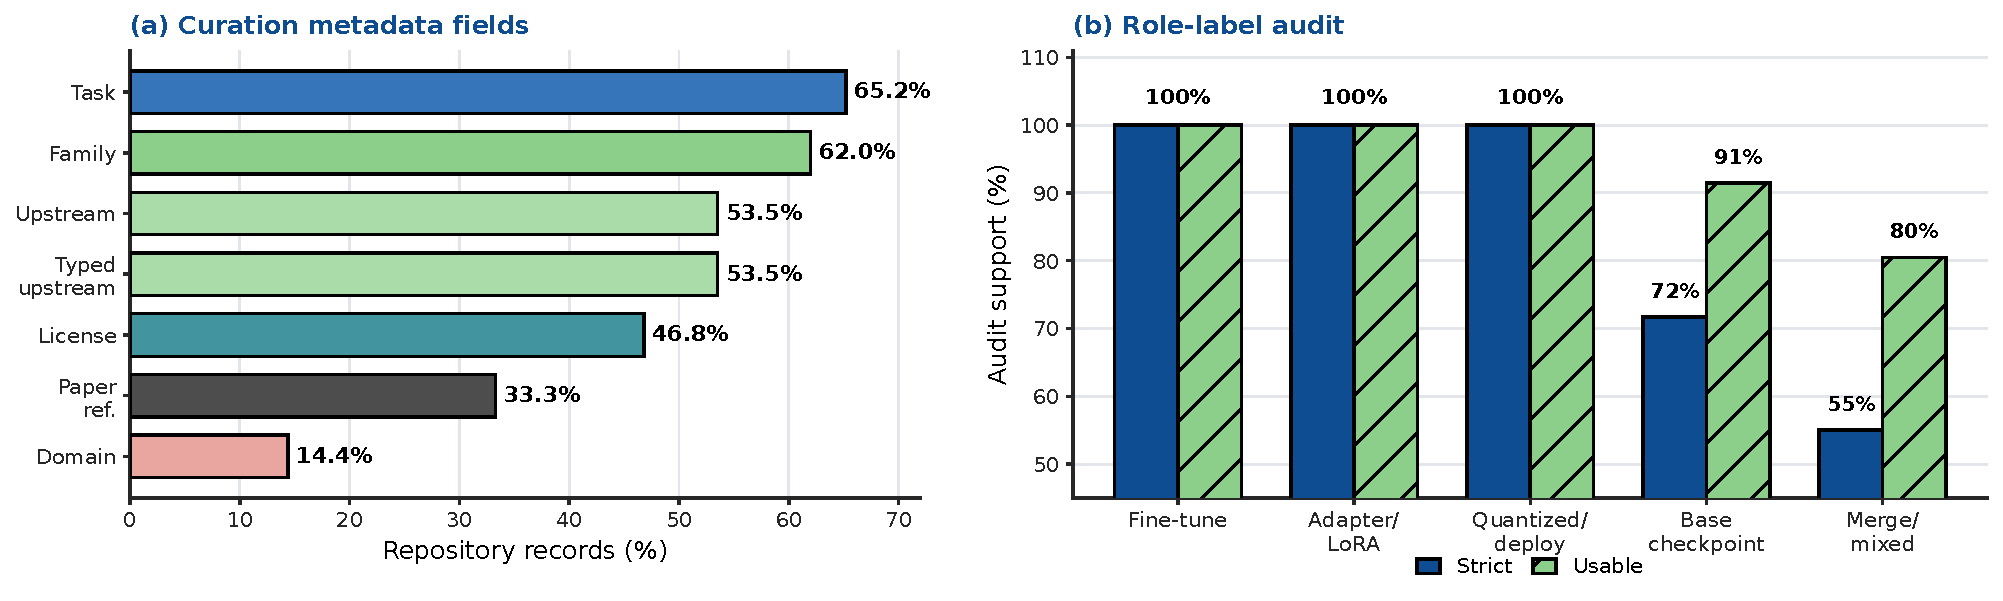
\includegraphics[width=\textwidth]{figures/fig2_metadata_completeness.pdf}
    \caption{Repository-side metadata coverage and role audit. Panel (a) reports curation-relevant metadata-field coverage across the fixed repository snapshot. Panel (b) shows balanced-audit support for role labels, separating strict support from usable support. Fine-tune, adapter, and quantized/deployment labels are stable in the audit sample; base and merge/mixed labels have lower strict support and wider ambiguity gaps.}
    \Description{A two-panel figure. The first panel is a horizontal bar chart of metadata-field coverage in repository records. The second panel is a grouped vertical bar chart comparing strict and usable audit support for five artifact-role labels.}
    \label{fig:metadata}
\end{figure*}

The balanced 300-repository expert audit finds 85.3\% overall strict role support (256/300; Wilson 95\% CI [80.9, 88.9]). Fine-tune, adapter/LoRA, and quantized/deployment records each reach 100.0\% strict support in the balanced sample (60/60 per class; lower Wilson bound 94.0\%). Base records have 71.7\% strict support (43/60; CI [59.2, 81.5]), and merge/mixed records have 55.0\% strict support (33/60; CI [42.5, 66.9]). These boundary classes are difficult because a repository can simultaneously carry base-family, merge, converted, or deployment signals; a single generic model label cannot capture that package structure.

For curation, the result is not that every repository has a single unambiguous identity. It is that public metadata can support a first typing layer if catalogs preserve both the primary artifact role and the package form, rather than collapsing base checkpoints, adapters, quantized files, merged models, and deployment packages into one generic model label. The next question is whether those typed repository records can be connected to the papers that introduce, use, or evaluate them.

\subsection{RQ2: What Bibliographic and Linkage Evidence Is Visible?}

The linkage break occurs between visible links and typed scholarly relations. GitHub or code-hosting links appear in 30.6\% of analysis-set paper records and \hf links in 10.5\%, yet matched paper-to-\hf repository evidence covers only 124 of 2,214 records, or 5.6\%. The problem is therefore not the absence of any link, but that links often lack a relation type: official release, dependency, baseline, example, or background reference.

Repository-side fields provide supporting context for linkage and discovery. Across the full snapshot, task descriptors appear in 65.2\% of repository records, model-family labels in 62.0\%, explicit upstream model fields in 53.5\%, typed upstream relation fields in 53.5\%, license tag signals in 46.8\%, scholarly references in 33.3\%, and domain descriptors in 14.4\%. These fields help organize a model collection, but they do not by themselves establish whether a repository is the artifact introduced by a paper, a dependency used by it, or a baseline cited for comparison.

The curation implication is that paper--repository relations should be typed. A record needs to distinguish whether a repository is introduced by the paper, used as a dependency, evaluated as a baseline, cited as background, or provided as an official release package. Once the relation is located, the next curation question is whether the public record also supports an upstream provenance claim.

\subsection{RQ3: What Level of Provenance Can Public Records Support?}

Public records often support family-level collection organization, while exact upstream claims require typed relation evidence. Figure~\ref{fig:provenance} separates upstream-evidence tiers from paper--repository alignment signals. Panel (a) shows that this pattern holds across mechanisms: exact matched paper--\hf anchors are consistently rare, while inventory-backed or weak family evidence is much more common. Panel (b) decomposes direct alignment signals used for bibliographic linkage; these signals are not treated as provenance unless the linked record exposes an upstream relation.

\begin{figure*}[!tbp]
    \centering
    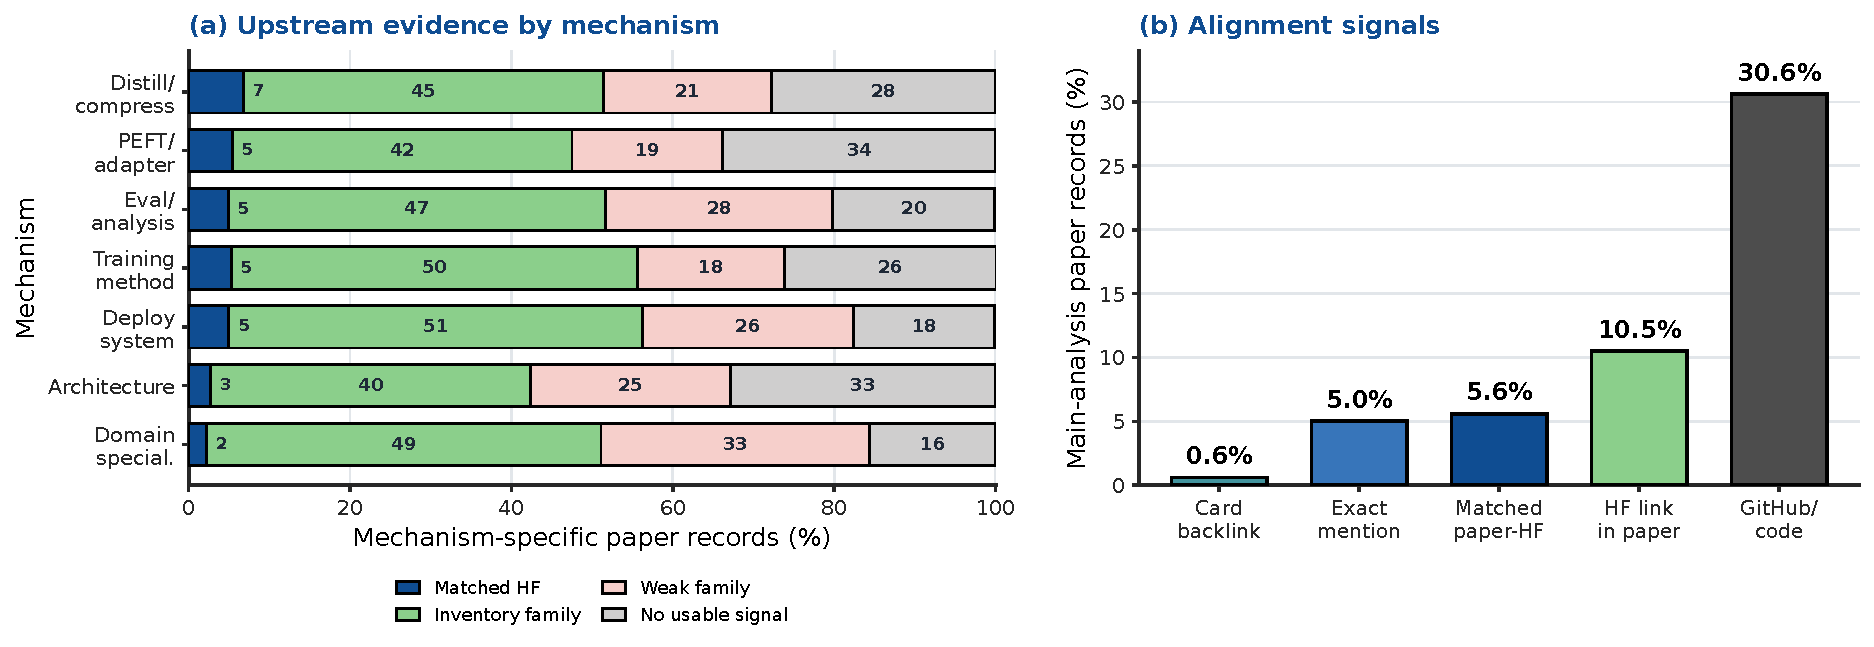
\includegraphics[width=\textwidth]{figures/fig3_provenance_alignment.pdf}
    \caption{Upstream-evidence tiers and paper--repository alignment signals. Panel (a) reports the strongest public-record anchor available for upstream or family-level interpretation by mechanism. Panel (b) ranks direct alignment signals for bibliographic linkage. Alignment signals support provenance only when the linked paper or repository exposes an upstream relation.}
    \Description{A two-panel figure. The first panel is a set of horizontal stacked bars showing upstream and family evidence tiers by research mechanism. The second panel is a vertical bar chart separating paper text links, matched model mentions, model-card backlinks, and the combined matched-link measure.}
    \label{fig:provenance}
\end{figure*}

Inventory-backed family signals cover 45.6\% of analysis-set paper records, weak or contextual family clues cover 21.9\%, and 26.9\% have no usable family or provenance signal. The expert upstream-evidence audit clarifies the strength of these signals: 28.0\% of 200 reviewed rows provide strict evidence for one clear primary upstream family (Wilson 95\% CI [22.2, 34.6]), while 79.0\% provide usable family-level support for collection-level grouping (CI [72.8, 84.1]). In curatorial terms, family evidence is often good enough for shelf placement, but not for a provenance claim.

The result supports a tiered provenance record. Family names are valuable for discovery and aggregate organization, but a curatable record should preserve whether the family appears as a base checkpoint, teacher, adapter target, merge input, quantization source, evaluator, baseline, or only background context. Provenance evidence identifies where an artifact comes from; release evidence determines what part of that artifact can actually be inspected or preserved.

\subsection{RQ4: What Release Package Evidence Is Visible?}

Release evidence is common at the statement level but much rarer at the asset-package level. Figure~\ref{fig:release}a reports the release-package distribution for the 2,214 analysis-set paper records. Overall, 32.8\% have no explicit release signal, 31.3\% have a stated or incomplete release signal, 24.3\% provide code, scripts, or recipe evidence, 6.8\% provide checkpoint or adapter evidence, less than 0.2\% provide data or evaluation asset evidence, and 4.5\% provide multiple assets or a full recipe.

\begin{figure*}[!tbp]
    \centering
    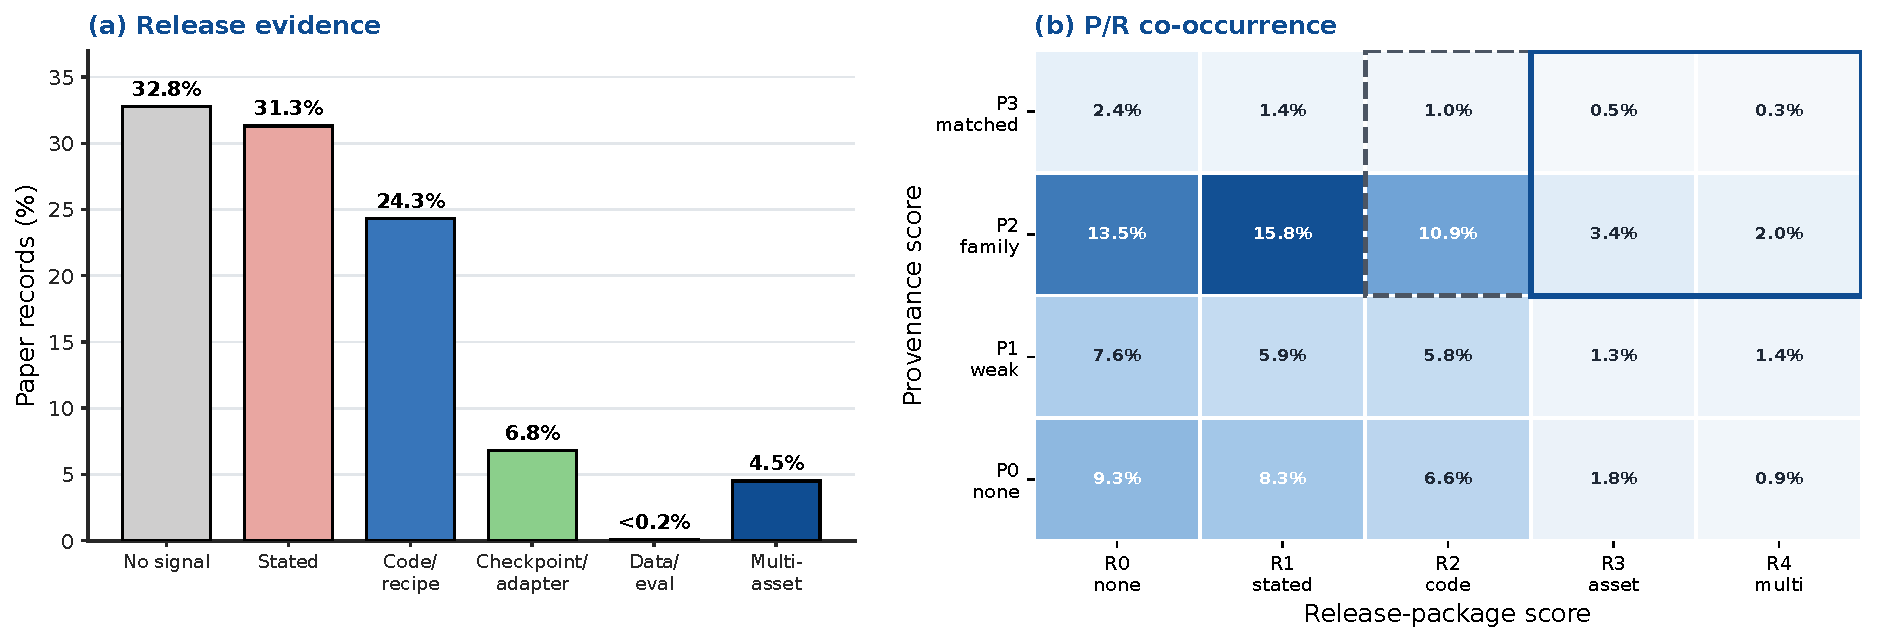
\includegraphics[width=\textwidth]{figures/fig4_release_curatability.pdf}
    \caption{Release evidence and provenance--release co-occurrence. Panel (a) shows release-package evidence by category. Panel (b) cross-tabulates provenance score $P$ and release-package score $R$ for the 2,214 analysis-set paper records; the dashed box marks the operational P+R region and the solid box marks the asset-level region used by the high-curatability threshold.}
    \Description{A two-panel figure. The first panel is a vertical bar chart for release evidence tiers. The second panel is a heatmap crossing provenance scores with release-package scores and highlighting the operational and high-curatability threshold regions.}
    \label{fig:release}
\end{figure*}

Collapsed into broader categories, 67.2\% contain some release or open-asset signal, 35.8\% contain concrete code or asset evidence, and 4.5\% contain strict multi-asset or full-recipe evidence. A targeted 50-row expert URL/asset-level audit found that all reviewed URL/asset assignments matched the visible public-evidence category; no aggregate category changes were required (50/50; Wilson 95\% CI [92.9, 100.0]).

The curation implication is that release should be recorded as a package, not as a binary availability flag. A paper can state that resources are released or expose GitHub scripts while still omitting weights, adapters, data, or evaluation assets; such a record helps inspection but does not yet provide an asset-level package. The final measurement asks how often provenance and release evidence appear together in the same paper record.

\subsection{RQ5: How Often Do the Required Evidence Fields Co-occur?}

The main bottleneck is combined curation readiness. Under the high-curatability threshold, a paper record must have usable provenance, asset-level or multi-asset release evidence, and at least one direct linkage signal. Only 136 of 2,214 analysis-set paper records satisfy this joint-evidence requirement, or 6.1\%.

Table~\ref{tab:key-results} reports the full threshold ladder. A broad discovery-ready rule covers 90.7\% of records. The operational P+R threshold, requiring usable provenance and code/recipe-or-stronger release evidence, covers 18.1\%. The high-curatability threshold covers 6.1\%, and the preservation-review threshold requiring multi-asset or full-recipe evidence covers 2.3\%. Figure~\ref{fig:release}b shows where the drop occurs in the provenance--release co-occurrence map: the operational region with $P\geq2$ and $R\geq2$ contains 401 records, but the asset-level region with $P\geq2$ and $R\geq3$ contains only 136 records.

The key diagnostic is the operational P+R subset. Among 401 records with both usable provenance and concrete release evidence, 400 also contain at least one direct linkage signal. The larger drop from 401 operational P+R records to 136 high-curatability records is therefore driven almost entirely by the release threshold: 265 operational records expose code, scripts, or recipes, but not an asset-level package such as a checkpoint, adapter, data, evaluation asset, or multi-asset recipe. In this corpus, the main bottleneck is not an isolated missing link after provenance and concrete release evidence are present. It is the co-occurrence of usable provenance with sufficiently concrete release assets.

This is the central empirical result: open \llm artifacts are broadly visible, but only a much smaller share expose enough coordinated evidence for provenance-aware curation. The funnel should therefore be read as an evidence-integration problem rather than an artifact-availability problem: the artifacts are often visible, but the record fields needed to justify curation claims are not yet coordinated.

\section{Discussion}
\label{sec:discussion}

The results show that compact and derived open \llm artifacts have entered the public scholarly record, but not yet as well-formed curation records. A curator looking at a paper and its public traces needs to answer four practical questions: What is the artifact? Which paper relation does the repository have? What upstream relation is evidenced? What assets can be inspected or preserved? The visibility-to-curatability funnel shows that these answers often exist separately, but rarely appear together in one typed record; after usable provenance and concrete release evidence are present, the remaining drop is driven mainly by whether the release evidence reaches the asset-package level. This section translates that gap into a minimal record design.

\subsection{From Visibility to a Minimal Curatable Record}

\begin{table*}[!tbp]
\centering
\caption{A minimal curatable record for compact and derived open \llm artifacts. The record acts as a coordination contract across existing systems rather than a requirement for a new centralized registry.}
\label{tab:minimal-curatable-record}
\small
\setlength{\tabcolsep}{4pt}
\renewcommand{\arraystretch}{1.12}
\begin{tabularx}{0.98\textwidth}{@{}p{0.15\textwidth}p{0.20\textwidth}p{0.22\textwidth}p{0.20\textwidth}Y@{}}
\toprule
Field group & Core field & Primary maintainer/source & Failure prevented & Curation use \\
\midrule
Artifact identity & \texttt{artifact\_role} & Model hub / repository owner & Generic model label & Catalog type \\
\rowcolor{TableGray}
Package form & \texttt{package\_form} & Model hub / repository metadata & Hidden distribution format & Package interpretation \\
Scholarly relation & \texttt{paper\_repository\_relation} & Paper authors + scholarly index & Untyped links & Bibliographic control \\
\rowcolor{TableGray}
Upstream relation & \texttt{upstream\_relation\_type} & Model hub + paper text & Family-as-provenance & Provenance relation \\
Evidence tier & \texttt{provenance\_evidence\_tier} & Digital library / index & Overstated confidence & Confidence and scope \\
\rowcolor{TableGray}
Release assets & \texttt{release\_asset\_types} & Model hub + code repository + paper & Release-as-binary & Asset package \\
License/access signal & \texttt{license\_access\_signal} & Model hub / repository metadata & Missing governance context & Access context \\
\bottomrule
\end{tabularx}
\renewcommand{\arraystretch}{1.0}
\end{table*}


Table~\ref{tab:minimal-curatable-record} summarizes the record that follows from the measurements. It is intentionally minimal: the fields correspond to the evidence needed to move from discovery to provenance-aware curation. Artifact role and package form describe what the object is and how it is distributed. Scholarly relation links the object to papers. Upstream relation and provenance-evidence tier separate family-level discovery from stronger derivation claims. Release assets describe what can be inspected or preserved. License and access signals add governance context that should accompany, but not replace, the integrated curatability status. The added failure-prevention column makes the design logic explicit: each field blocks a specific ambiguity observed in the audit or funnel.

The table also shows that the record can be assembled as a coordination layer across existing infrastructure, provided that stable identifiers, bidirectional links, typed relation fields, release-asset fields, and versioned evidence tiers are preserved. Model hubs and repository owners are closest to artifact role, package form, upstream relation, release assets, and license metadata. Paper authors and scholarly indexes are closest to paper--repository relations. Digital libraries and preservation systems are positioned to store evidence tiers and curation-readiness status because they integrate records from multiple sources.

This design is intentionally modest. It does not require a single authority to certify every open-model artifact. Instead, it asks each infrastructure layer to expose the relation it is already closest to: model hubs expose artifact and release structure, scholarly indexes expose paper relations, and digital libraries preserve evidence tiers across systems. The result is not a heavier publication burden, but a record that makes existing public traces usable for citation, attribution, reuse assessment, and preservation triage.

The boundary cases observed in the audits explain why the fields should remain typed. A family name can mark a target model, parent, teacher, baseline, evaluator, or false positive context match. A GitHub link can expose scripts without weights. A \hf link can identify a dependency or checkpoint without an asset-level release package. These traces are useful, but they are not interchangeable. A curation record should preserve their relation type and evidentiary strength rather than compressing them into a generic ``open model'' label.

\subsection{Infrastructure Responsibilities and Design Implications}

The funnel suggests a practical division of labor. Because release assets and full recipes are rare, \textbf{model hubs} are the natural place to maintain artifact-role, package-form, upstream-relation, release-asset, and license/access fields close to the artifact. Because matched paper--\hf repository evidence covers only 5.6\% of paper records, \textbf{scholarly indexes} should type paper--repository relations rather than storing unqualified links. Because family evidence is often usable for grouping but weak for strict upstream claims, \textbf{digital libraries and preservation systems} should preserve provenance-evidence tiers and curation-readiness status across sources. The priority is not a new registry of every model artifact, but a coordination layer that keeps existing public traces joinable without losing their source or evidentiary strength.

This division of labor leads to five evidence-to-action interventions.
\begin{enumerate}[leftmargin=*,itemsep=2pt,topsep=2pt]
    \item \textbf{Role ambiguity $\rightarrow$ separate artifact role from package form.} Model hubs should distinguish base checkpoints, fine-tunes, adapters, merges, quantized files, and deployment packages without forcing them into one generic model label.
    \item \textbf{Sparse direct linkage $\rightarrow$ type paper--repository relations.} Scholarly indexes should distinguish repositories introduced by a paper, used as dependencies, evaluated as baselines, cited as background, or provided as official release packages.
    \item \textbf{Family-as-provenance risk $\rightarrow$ type upstream relations.} Model records should distinguish base, teacher, adapter target, merge input, quantization source, evaluator, baseline, and background mention relations.
    \item \textbf{Uneven evidence strength $\rightarrow$ represent provenance tiers.} Digital libraries should preserve whether a claim rests on an explicit upstream field, a matched repository with a visible upstream relation, an inventory-backed family signal, or a contextual mention.
    \item \textbf{Binary release labels $\rightarrow$ expose release packages as structured fields.} Release records should separate code, scripts, weights or checkpoints, adapters, datasets, evaluation assets, recipes, and environment details.
\end{enumerate}

These interventions align with FAIR software and research-object packaging work, which treats reuse as a property of structured packages and relations rather than of a single access flag \cite{barker2022fair4rs,soilandreyes2022rocrate}. The Model Openness Framework makes a related point at the level of openness components \cite{white2024mof}. The contribution here is empirical and record-level: open \llm artifacts are often visible, but digital-library infrastructure should make the evidence needed for citation, provenance tracking, reuse assessment, and preservation selection explicit, typed, and actionable.

\section{Scope and Limitations}
\label{sec:limitations}

These limitations define the scope of the public-record claims rather than weakening the main result. The repository collection is a May 2026 \hf snapshot scoped to compact and derived open \llm artifacts, not a census of every \hf repository. The paper corpus is a constructed scholarly record set; main percentages use 2,214 analysis-set paper records unless otherwise stated. Artifact role and package form are audited inference fields derived from public metadata, with stronger support for fine-tune, adapter/LoRA, and quantized/deployment records than for base and merge/mixed records. Provenance tiers measure public upstream evidence; they do not recover private training logs, hidden checkpoints, or developer knowledge. Release-package evidence records visible assets, but execution, environment reconstruction, model quality, adoption, and preservation success remain downstream tasks.

\section{Conclusion}
\label{sec:conclusion}

This paper contributes a record-design measurement framework for compact and derived open \llm artifacts. These artifacts are becoming a distributed digital collection represented across model hubs, model cards, scholarly papers, code repositories, family mentions, release statements, and paper--repository links. Linking a fixed \hf repository snapshot with scholarly paper records shows that broad visibility is common, but coordinated evidence is much rarer: 90.7\% of paper records are discovery-ready, 18.1\% meet the operational P+R threshold, 6.1\% satisfy the high-curatability threshold, and 2.3\% qualify as preservation-review candidates.

The implication for digital libraries is concrete. Open-model infrastructure should expose typed artifact roles, package-form fields, upstream relation types, provenance-evidence tiers, bidirectional paper--repository links, and release-package fields. These interventions shift the question from whether open \llm artifacts are online to whether public records can justify curation decisions about attribution, traceability, reuse assessment, and preservation triage. The next generation of open-model infrastructure should not only keep artifacts online; it should keep the evidence around those artifacts connected.


\bibliographystyle{ACM-Reference-Format}
\bibliography{references}

\end{document}
